%% AMS-LaTeX Created by Wolfram Mathematica 7.0 : www.wolfram.com
\documentclass[letterpaper,12pt,final,titlepage]{article}
%PREAMBLE:
\usepackage[total={18cm,21cm},top=2cm, left=2cm]{geometry} %simplifica la definici�n de margenes
\usepackage[leqno]{amsmath}
\usepackage{latexsym}
\usepackage{amsmath, amssymb, graphics}
\usepackage{color} %agregar color a las partes del documento que se prefieran%
\usepackage[spanish,activeacute]{babel}
\usepackage[latin1]{inputenc}
\usepackage{setspace}
\usepackage[pdftex]{graphicx}
\usepackage{epstopdf}
\usepackage{graphicx} %sirve para insertar graficos en varios formatos%
\usepackage{epsfig,tocbibind}%para incluir figuras en .EPS de Stata
\usepackage{fancyhdr} %agrega topes y pies de pagina%
\usepackage{rotating} %por si quiero colocar un hoja horizontal
\usepackage{anysize} %sirve para definir margenes%
\usepackage{hyperref} %para crear enlaces dentro del propio documento o para insertar urls.
\usepackage[sort]{natbib} % Reference List
\usepackage{tabulary}
\usepackage{tabularx}
\usepackage{afterpage}
\newcommand{\mathsym}[1]{{}}
\newcommand{\unicode}{{}}

%%%%%%%%%%%%%%%%%%%%%%%%%%%%%%%%%%%%%%%%%%%%%%%%%%%%%%%%%%%%%%%%%%%%%%%%%%%%%%%%%%

\begin{document}
\begin{center}
\begin{large}
\textbf{Taller econometr�a (EC402) n�mero \#4:}
\end{large}\\
\textbf{Prof. Andr�s Mauricio Casta�o Zuluaga}
\end{center}
\bigskip

\textbf{1. A continuaci�n se van a mostrar distintas especificaciones de una regresi�n lineal multiple para los factores determinates del salario promedio por hora trabajada (sxh) de los trabajadores a nivel comunal en chile (en pesos). Los variables explicativas utilizadas van a ser:}

\begin{itemize}
\item Escolaridad  promedio de los trabajadores de cada comuna, medida en a�os promedio (esc)
\item Experiencia promedio de los trabajadores de cada comuna, medida en a�os promedio (exper)
\item Experiencia al cuadrado promedio de los trabajadores de cada comuna, medida en a�os promedio (exper2)
\item Poblaci�n de cada comuna, medida en miles de habitantes por comuna (populationc)
\item Tasa de desocupaci�n de cada comuna, medida en \% (tdocc)
\end{itemize}

\textbf{Realize lo siguiente:}
\begin{itemize}
\item 1. Interprete los coeficientes de cada uno de los distintos modelos (de acuerdo a su especificaci�n), tienen sentido desde la teor�a econ�mica cada uno de los signos obtenidos, justifique su respuesta.
\item 2. Determine la significancia individual y global del modelo.
\item 3. Interprete los intervalos de confianza y la medida de bondad de ajuste, �podr�a predecir este modelo de buena manera el comportamiento de los salarios a nivel comunal?.
\item 4. Para el caso de la regresi�n estandarizada, obtenga los coeficientes expresados en la �ltima columna e interpretelos, �cual es la variable explicativa que mayor impacto tiene sobre el salario por hora a nivel comunal?
\end{itemize}


\begin{center}
\begin{figure}[!ht]
\centering
\caption{\textbf{Resultados estimaci�n ecuaci�n de salarios a nivel comunal en chile, modelo normal.}}
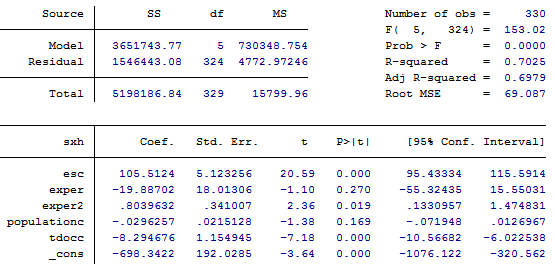
\includegraphics[width=15cm]{Modelo_normal}
\end{figure}
\end{center}

\begin{center}
\begin{figure}[!ht]
\centering
\caption{\textbf{Resultados estimaci�n ecuaci�n de salarios a nivel comunal en chile, modelo con coeficientes estandarizados.}}
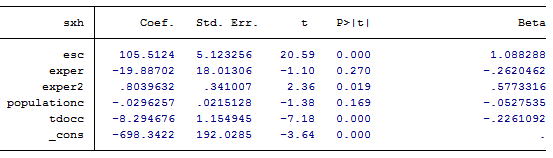
\includegraphics[width=15cm]{Modelo_Estandarizado}
\end{figure}
\end{center}

\begin{center}
\begin{figure}[!ht]
\centering
\caption{\textbf{Resultados estimaci�n ecuaci�n de salarios a nivel comunal en chile, modelo log-log.}}
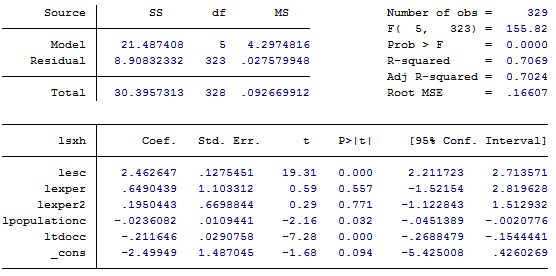
\includegraphics[width=15cm]{modelo_log-log}
\end{figure}
\end{center}

\begin{center}
\begin{figure}[!ht]
\centering
\caption{\textbf{Resultados estimaci�n ecuaci�n de salarios a nivel comunal en chile, modelo log-lin.}}
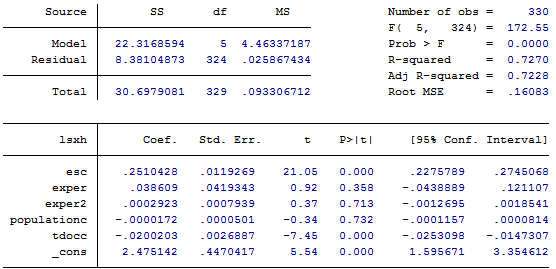
\includegraphics[width=15cm]{Modelo_log-lin}
\end{figure}
\end{center}


\begin{center}
\begin{figure}[!ht]
\centering
\caption{\textbf{Resultados estimaci�n ecuaci�n de salarios a nivel comunal en chile, modelo lin-log.}}
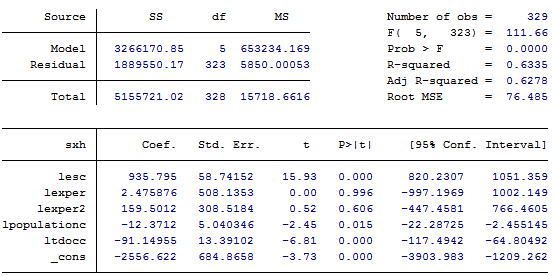
\includegraphics[width=15cm]{Modelo_lin-log}
\end{figure}
\end{center}

\end{document} 